\chapter{گام 3: مدل‌سازی ناحیه حفاطت شده و فیلتر کردن توالی‌ها }
            در این مرحله هدف ساخت یک مدل برای ناحیه حفاظت شده طولانی‌ترین توالی زیر خانواده thermostable از زاینالازها است.
        \section{دیدگاه کلی}
            در فرآیند شناسایی آنزیم‌های زایلاناز کاربردی از مجموعه داده‌های متاژنومی، مرحله 3 نقش مهمی در پالایش و اعتبارسنجی توالی‌های شناسایی‌شده در مراحل قبلی دارد. هدف کلی این مرحله تجزیه و تحلیل مناطق حفاظت شده در توالی های خوشه ای و فیلتر کردن نامزدهای کمتر قابل اعتماد است و اطمینان حاصل می کند که فقط مرتبط ترین توالی ها برای تجزیه و تحلیل پایین دست باقی می مانند. این مرحله بر تکنیک‌های محاسباتی پیشرفته، از جمله ماتریس‌های امتیازدهی خاص موقعیت (PSSM) و مدل‌های مارکوف پنهان (HMMs)، برای شناسایی موتیف‌های حفاظت‌شده، امتیاز مربوط به ترتیب و حذف توالی‌های اضافی یا کم‌اعتماد متکی است.

            در زمینه مطالعات متاژنومیک، توالی‌های بیولوژیکی بازیابی شده از نمونه‌های محیطی اغلب دارای تغییرات قابل‌توجهی به دلیل جهش، واگرایی تکاملی و خطاهای توالی هستند. با این حال، پروتئین های حیاتی عملکردی، مانند آنزیم های دخیل در تخریب زیست توده، معمولاً باقیمانده های بسیار حفاظت شده را در مناطق کاتالیزوری و اتصال به بستر خود حفظ می کنند. این حوزه های حفاظت شده برای عملکرد مناسب آنزیم اساسی هستند، زیرا یکپارچگی ساختاری و کارایی کاتالیزوری را تضمین می کنند. بنابراین، مدل‌سازی این نواحی و فیلتر کردن توالی‌هایی که حاوی موتیف‌های به خوبی محافظت‌شده نیستند، برای به حداکثر رساندن احتمال شناسایی زایلانازهای کاربردی واقعی ضروری است.

            یکی دیگر از جنبه های مهم مرحله 3، استفاده از فیلترینگ توالی برای حذف توالی هایی است که معیارهای حفاظت را برآورده نمی کنند. با پالایش مجموعه داده، این فرآیند دقت تجزیه و تحلیل های پایین دستی مانند حاشیه نویسی عملکردی، پیش بینی ساختار پروتئین و خصوصیات بیوشیمیایی را بهبود می بخشد. بدون این فیلتر، خطر بیشتری برای انتشار توالی های اشتباه وجود دارد که می تواند تلاش های اعتبارسنجی آزمایشی بعدی را به خطر بیندازد. بنابراین، این مرحله به عنوان یک نقطه بازرسی کنترل کیفیت عمل می‌کند و قابلیت اطمینان توالی‌های کاندید زایلاناز را برای بررسی بیشتر تقویت می‌کند.

            با استفاده از 
            PSI-BLAST 
            برای ایجاد مدل‌های 
            PSSM 
            و 
            HMMER 
            برای تولید مدل‌های مارکوف پنهان، این مرحله چارچوبی قدرتمند برای تشخیص الگوهای حفاظت از توالی فراهم می‌کند. این رویکردهای محاسباتی به طور گسترده در بیوانفورماتیک برای شناسایی همولوگ های راه دور، پیش بینی مکان های عملکردی و افزایش درک ما از تکامل آنزیم استفاده می شود. نتایج این مرحله نه تنها مجموعه داده‌ها را اصلاح می‌کند، بلکه بینشی در مورد چگونگی تکامل آنزیم‌های زایلاناز و سازگاری با شرایط مختلف محیطی، به‌ویژه در جوامع میکروبی گرمادوست، ارائه می‌کند.
        \section{زمینه علمی: دامنه های حفاظت شده و نقش آنها در عملکرد زایلاناز}
            دامنه‌های حفاظت‌شده نواحی خاصی در توالی‌های پروتئینی هستند که به دلیل نقش اساسی در عملکرد آنزیمی و پایداری ساختاری، در بین گونه‌های مختلف بسیار حفظ می‌شوند. این دامنه ها اغلب حاوی باقیمانده هایی هستند که برای فعالیت کاتالیزوری، اتصال به بستر یا برهمکنش های پروتئین-پروتئین ضروری هستند. وجود دامنه‌های حفاظت‌شده در یک توالی پروتئین نشان می‌دهد که پروتئین نقش عملکردی خود را در طول تکامل حفظ کرده است و آن را به یک کاندیدای قوی برای مطالعه بیشتر تبدیل می‌کند.

            برای آنزیم‌های زایلاناز، حوزه‌های حفاظت‌شده از اهمیت ویژه‌ای برخوردار هستند، زیرا مکانیسم هیدرولیز زایلان را تعریف می‌کنند. زایلانازها به خانواده گلیکوزید هیدرولاز (GH) تعلق دارند که اکثر اعضای مشخصه آن در میان سایرین تحت GH10 و GH11 قرار دارند. این آنزیم ها تجزیه زایلان، جزء اصلی همی سلولز گیاهی را با شکستن پیوندهای بتا-1،4-گلیکوزیدی کاتالیز می کنند. عملکرد کاتالیزوری زایلاناز به شدت به بقایای حفاظت شده خاص، از جمله باقی مانده های اسیدی (اسید آسپارتیک و اسید گلوتامیک) وابسته است که به عنوان دهنده پروتون و نوکلئوفیل در طول واکنش برش آنزیمی عمل می کنند.
            
            ساختار زایلانازها بسته به خانواده GH اغلب شامل یک دامنه کاتالیزوری با یک چین آلفا/بتا بشکه یا یک چین بتا-ژلیلول است. این نقوش ساختاری برای شناسایی و کاتالیز سوبسترا بسیار مهم هستند، به این معنی که تغییرات در این مناطق می تواند به شدت فعالیت آنزیم را تغییر دهد. با تجزیه و تحلیل دامنه های حفاظت شده در توالی های زایلاناز، پیش بینی عملکرد آنزیمی حتی در پروتئین های تازه کشف شده یا قبلاً مشخص نشده ممکن می شود. علاوه بر این، وجود ماژول‌های اتصال کربوهیدرات اضافی (CBM) می‌تواند ویژگی سوبسترا را افزایش دهد و بر عملکرد آنزیم در کاربردهای صنعتی تأثیر بگذارد.
            
            با توجه به اینکه زایلانازها به طور گسترده در تولید سوخت زیستی، صنعت کاغذ، خوراک دام و فرآوری مواد غذایی استفاده می‌شوند، شناسایی انواع بسیار پایدار و کارآمد ضروری است. بسیاری از زایلانازهای طبیعی برای شرایط محیطی خاص، مانند دماهای بالا، pH شدید، یا تحمل نمک بهینه شده اند. از طریق مدل‌سازی منطقه حفاظت‌شده، محققان می‌توانند سازگاری‌های ساختاری را مشخص کنند که به زایلانازهای خاصی اجازه می‌دهد در شرایط شدید عمل کنند و آنها را کاندیدای عالی برای کاربردهای بیوتکنولوژیکی می‌کند.
            
            اهمیت تجزیه و تحلیل دامنه حفاظت شده فراتر از مقایسه توالی ساده است. با شناسایی الگوهای حفاظت، محققان می توانند روابط تکاملی را ردیابی کنند، ویژگی بالقوه بستر را استنباط کنند، و حتی استراتژی های مهندسی آنزیم را برای افزایش خواص کاتالیزوری طراحی کنند. شناسایی و توصیف مناطق حفاظت‌شده، کشف انواع زایلاناز جدید با پایداری و کارایی بهبود یافته را امکان‌پذیر می‌سازد، که باعث پیشرفت در بیوتکنولوژی صنعتی و زیست‌شناسی مصنوعی می‌شود.

    \textbf{نواحی حفاظت‌شده} در زایلانازها به نواحی از توالی پروتئینی گفته می‌شود که در طی تکامل به‌طور نسبتاً ثابت باقی مانده‌اند و تغییرات کمی در آن‌ها رخ داده است. این نواحی معمولاً عملکردهای ضروری آنزیم، مانند سایت‌های فعال و ساختارهای فضایی آنزیم را نگه می‌دارند و در نتیجه برای عملکرد صحیح آنزیم ضروری هستند.

    در پروژه‌های زیستی و بایوانفورماتیک، انتخاب روش مناسب برای مدل‌سازی توالی‌ها و نواحی حفاظتی نقش بسیار مهمی در دقت و کارایی نتایج دارد. در این بخش، به هر دو روش پرکاربرد در مدل‌سازی توالی‌ها، یعنی ماتریس امتیازدهی موقعیت-ویژه (PSSM) و مدل‌های مخفی مارکوف (HMM)، پرداخته خواهد شد.


        \section{Multiple Sequence Alignment (MSA) Using Clustal Omega}
            \subsection{هدف MSA}
                تراز چند توالی 
                (MSA) 
                یک تکنیک اساسی بیوانفورماتیک است که برای هم‌ترازی مجموعه‌ای از توالی‌های بیولوژیکی برای شناسایی مناطق مشابه استفاده می‌شود. این شباهت ها اغلب روابط ساختاری، عملکردی یا تکاملی بین دنباله ها را نشان می دهد. در زمینه توالی های پروتئین زیلاناز، 
                MSA 
                برای تشخیص باقی مانده های بسیار حفاظت شده که احتمالا برای عملکرد آنزیمی حیاتی هستند ضروری است.

                هدف کلیدی انجام 
                MSA 
                در این مرحله آنالیز نواحی حفاظت‌شده در میان توالی‌های نماینده به‌دست‌آمده از مرحله 2 است. از آنجایی که زایلانازها متعلق به خانواده‌های گلیکوزید هیدرولاز با مشخصه‌های خوبی هستند 
                (مانند GH10، GH11)، 
                حوزه‌های کاتالیزوری، محل‌های اتصال و نقوش ساختاری آن‌ها باید در گونه‌های مختلف محافظت شوند. با تراز کردن این توالی‌ها، می‌توانیم بقایای حیاتی را که برای فعالیت آنزیمی و ثبات ساختاری ضروری هستند، مشخص کنیم.
                
                علاوه بر این، MSA امکان پیش‌بینی عملکردی بر اساس حفظ توالی را فراهم می‌کند. باقیمانده‌های بسیار حفاظت‌شده اغلب با بقایای کاتالیزوری، نقوش اتصال به بستر یا مکان‌های تثبیت ساختاری مطابقت دارند. اگر یک باقیمانده خاص به شدت در چندین توالی حفظ شود، به شدت نقش عملکردی را نشان می دهد. برعکس، مناطق متغیر ممکن است سازگاری هایی را نشان دهند که به آنزیم های زایلاناز اجازه می دهد در شرایط محیطی مختلف عمل کنند.
                
                انجام 
                MSA 
                همچنین ایجاد مدل‌های آماری مانند ماتریس‌های امتیازدهی خاص موقعیت 
                (PSSM) 
                و مدل‌های پنهان مارکوف 
                (HMMs) 
                را ممکن می‌سازد، که در مراحل بعدی برای اصلاح فیلترینگ توالی استفاده می‌شوند. این مدل‌ها به تشخیص تغییرات دنباله‌ای ظریف و در عین حال حفظ نقوش مرتبط بیولوژیکی کمک می‌کنند. بدون 
                MSA 
                مناسب، فرآیندهای پایین دستی مانند تشخیص دامنه حفاظت شده، پیش بینی ساختار و حاشیه نویسی عملکردی به طور قابل توجهی کمتر قابل اعتماد خواهند بود.
                
                بنابراین، 
                MSA 
                به عنوان یک مرحله پیش پردازش حیاتی عمل می کند که دقت پیش بینی های عملکردی مبتنی بر توالی را افزایش می دهد. این تضمین می‌کند که فقط توالی‌های مرتبط با بیولوژیک به مراحل بعدی تجزیه و تحلیل می‌روند و در عین حال توالی‌های نامرتب، اضافی یا غیرعملکردی را حذف می‌کنند.
            \subsection*{اجرای Omega Clustal}
                برای انجام MSA، ما از Clustal Omega، یک ابزار پرکاربرد MSA که به دلیل کارایی و دقت آن شناخته شده است، استفاده می کنیم.
                \begin{figure}[H]
                    \centering
                    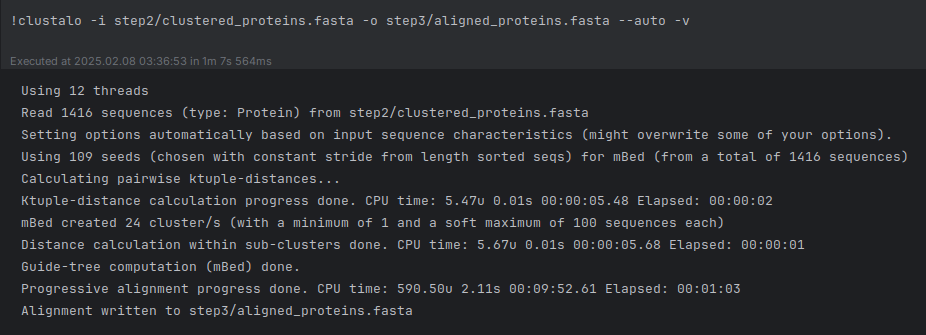
\includegraphics[width=0.8\textwidth]{images/run_omega_clustal.png} % Replace with your image file
                    \caption{اجرای Omega Clustal}
                    \label{fig:run_omega_clustal}
                \end{figure}
                فایل ورودی، step2/clustered\_proteins.fasta، حاوی توالی های نماینده استخراج شده از خوشه بندی CD-HIT است. از آنجایی که خوشه‌بندی باعث کاهش افزونگی در مرحله 2 شد، توالی‌های ارائه‌شده به Clustal Omega از قبل غیراضافی بودند و فرآیند هم‌ترازی را کارآمدتر و دقیق‌تر می‌کردند.

                پس از اجرای Clustal Omega، توالی های تراز شده در step3/aligned\_proteins.fasta ذخیره شدند. این فایل به عنوان ورودی حیاتی برای مدل‌سازی توالی بیشتر، از جمله ایجاد PSSM (PSI-BLAST) و تولید HMM (HMMER) عمل می‌کند.

                پس از اجرا، Clustal Omega با موفقیت 1948 توالی پروتئین را که مربوط به تعداد خوشه های تولید شده در مرحله 2 است، تراز کرد. هم ترازی تقریباً در 5 دقیقه تکمیل شد و کارایی Clustal Omega را در مدیریت مجموعه داده های بزرگ نشان داد.

        \section{ایجاد یک پایگاه داده BLAST برای جستجوی منطقه حفاظت شده}
            \subsection*{چرا یک پایگاه داده BLAST ایجاد کنیم؟}
                یکی از مراحل حیاتی در شناسایی مناطق حفاظت شده در توالی های زایلاناز، ایجاد پایگاه داده BLAST است که جستجو و مقایسه توالی کارآمد را تسهیل می کند. هدف اولیه از ساخت پایگاه داده BLAST، ذخیره توالی های خوشه ای زایلاناز در قالبی است که امکان جستجوی شباهت سریع با استفاده از PSI-BLAST و سایر ابزارهای مبتنی بر BLAST را فراهم کند. این فرآیند برای شناسایی توالی‌های همولوگ، شناسایی حفاظت تکاملی، و فیلتر کردن توالی‌ها بر اساس ارتباط عملکردی آنها بسیار مهم است.

                در مطالعات متاژنومی، مجموعه داده ها اغلب حاوی هزاران دنباله با درجات مختلف شباهت هستند. روش‌های هم‌ترازی توالی زوجی سنتی مانند Clustal Omega برای مجموعه داده‌های کوچک مؤثر هستند، اما وقتی با مجموعه داده‌های متاژنومی در مقیاس بزرگ سروکار دارند، از نظر محاسباتی گران می‌شوند. یک پایگاه داده BLAST با ارائه یک فضای جستجوی از پیش نمایه شده، که امکان مقایسه سریع و مقیاس پذیر توالی را فراهم می کند، بر این محدودیت غلبه می کند. با ساختاردهی توالی‌های زایلاناز خوشه‌ای در یک پایگاه داده BLAST، می‌توانیم به طور موثر توالی‌های جدید را در برابر مجموعه داده‌های موجود پرس‌وجو کنیم تا تعیین کنیم که چقدر با انواع زایلاناز شناخته شده مطابقت دارند.

                یکی دیگر از مزایای کلیدی ایجاد پایگاه داده BLAST این است که تجزیه و تحلیل منطقه حفاظت شده را امکان پذیر می کند. از آنجایی که باقیمانده‌های مهم عملکردی در بین توالی‌های همولوگ بسیار حفظ می‌شوند، استفاده از پایگاه داده BLAST به ما امکان می‌دهد تا برای نقوش حفاظت‌شده در تمام پروتئین‌های زایلاناز شناسایی‌شده جستجو کنیم. این به ویژه در تولید ماتریس امتیازدهی ویژه موقعیت (PSSM) مفید است، جایی که توالی‌هایی که با مناطق حفاظت‌شده با اطمینان آماری بالا مطابقت دارند، حفظ می‌شوند، در حالی که توالی‌های با اعتماد پایین فیلتر می‌شوند.

                به طور خلاصه، یک پایگاه داده BLAST به عنوان یک مخزن متمرکز از توالی‌های زایلاناز خوشه‌ای عمل می‌کند، که امکان جستجوی سریع تشابه، تشخیص منطقه حفاظت‌شده، و فیلتر کردن توالی با اطمینان بالا را فراهم می‌کند. بدون پایگاه داده BLAST، مقایسه‌های توالی به طور قابل‌توجهی کندتر و مقیاس‌پذیرتر خواهند بود، و شناسایی مناطق مهم عملکردی در مجموعه داده‌های متاژنومی بزرگ را به چالش می‌کشد.
            \subsection*{دستور MakeBLASTDB}
                برای ایجاد یک پایگاه داده BLAST از توالی های خوشه ای زایلاناز، از دستور makeblastdb استفاده می کنیم که بخشی از مجموعه NCBI BLAST+ است. این دستور یک فایل FASTA را به یک پایگاه داده سازگار با BLAST تبدیل می کند و امکان جستجوی توالی کارآمد را فراهم می کند.
                \begin{figure}[H]
                    \centering
                    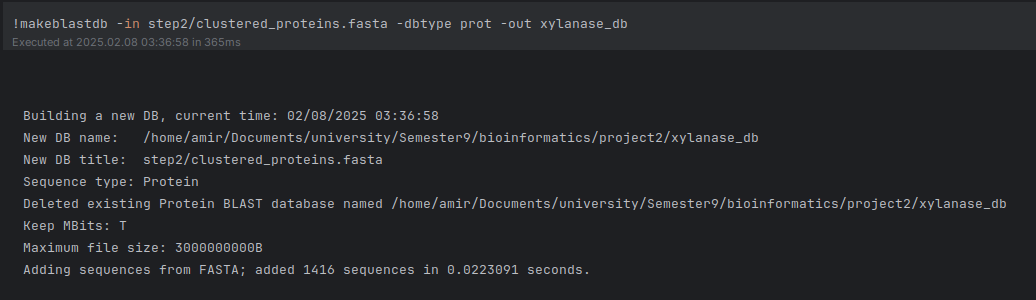
\includegraphics[width=0.8\textwidth]{images/make_blast.png} % Replace with your image file
                    \caption{اجرای make blast}
                    \label{fig:make_blast}
                \end{figure}

                ایجاد موفقیت آمیز پایگاه داده BLAST یک گام مهم به سمت تجزیه و تحلیل توالی زایلاناز با اطمینان بالا است. با ساختاربندی توالی‌های خوشه‌بندی‌شده در قالبی قابل جستجو، کارایی جستجوهای تشابه توالی، شناسایی دامنه حفظ‌شده و عملکردی را بهبود بخشیده‌ایم. پایگاه داده اکنون به عنوان یک منبع حیاتی برای پالایش انتخاب توالی، فیلتر کردن نامزدهای کم اعتماد، و اطمینان از اینکه فقط دنباله‌های مرتبط با عملکرد به مراحل بعدی ادامه می‌دهند، عمل می‌کند.

                با حرکت رو به جلو، این پایگاه داده BLAST برای تکرارهای PSI-BLAST استفاده خواهد شد، که یک مدل PSSM را برای اصلاح تجزیه و تحلیل حفظ توالی ایجاد می کند. علاوه بر این، از آن در تشخیص موتیف مبتنی بر 
                HMMER 
                استفاده خواهد شد.

                با ایجاد پایگاه داده، گام بعدی شامل استفاده از PSI-BLAST و HMMER برای استخراج توالی های حفاظت شده با اطمینان بالا خواهد بود و اطمینان حاصل می کند که مرتبط ترین کاندیدهای زایلاناز از نظر بیولوژیکی برای مطالعه بیشتر شناسایی می شوند.
        \section{ماتریس 
        \lr{PSSM (Position-Specific Scoring Matrix)}}
            ماتریس PSSM  یا ماتریس امتیازدهی موقعیت-ویژه ابزاری برای توصیف الگوهای خاص در توالی‌های زیستی مانند پروتئین‌ها و DNA است. این ماتریس، احتمال جایگزینی هر اسیدآمینه (یا نوکلئوتید در مورد DNA) را در هر موقعیت مشخص از یک توالی نشان می‌دهد.
            \subsubsection*{اجرای PSI-BLAST}
            برای تولید یک PSSM برای توالی‌های زایلاناز، از PSI-BLAST برای اصلاح مکرر ماتریس امتیازدهی استفاده شد. دستور زیر اجرا شد:
            \begin{figure}[H]
                \centering
                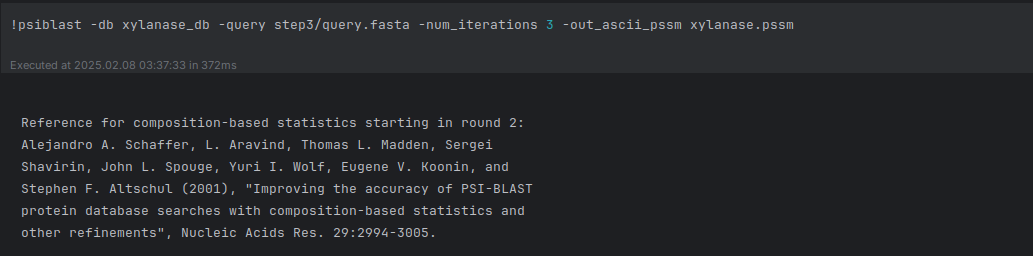
\includegraphics[width=0.8\textwidth]{images/run_psiblast.png} % Replace with your image file
                \caption{اجرای run psiblast}
                \label{fig:run_psiblast}
            \end{figure}

            \subsubsection*{ساختار ماتریس  PSSM}
            در ماتریسی که ارائه داده‌ای، هر سطر نمایانگر یک موقعیت خاص در توالی پروتئینی است و هر ستون نماینده یکی از ۲۰ اسیدآمینه استاندارد 
            \lr{( A، C، D، E، F، ...، Y)} 
            می‌باشد. هر مقدار درون این ماتریس، یک امتیاز عددی است که بیانگر احتمال (یا تمایل) جایگزینی آن اسیدآمینه در موقعیت موردنظر است.
            \begin{itemize}
                \item مقادیر مثبت $\leftarrow$ نشان‌دهنده تمایل بالاتر یک اسیدآمینه خاص به حضور در موقعیت موردنظر
                \item مقادیر منفی $\leftarrow$ نشان‌دهنده عدم تمایل (یا نادر بودن) یک اسیدآمینه در آن موقعیت
            \end{itemize}

            در ماتریس محاسبه شده، مقدار -19.931569 اغلب تکرار شده است که ممکن است نشان‌دهنده یک مقدار حداقلی پیش‌فرض باشد. مقدار -10.768146  در برخی نقاط دیده می‌شود که احتمالاً نشان‌دهنده اسیدآمینه‌هایی است که به‌صورت ضعیف‌تر ولی قابل توجه در آن موقعیت رخ داده‌اند.

            \begin{figure}[H]
                \centering
                \begin{subfigure}[b]{0.4\textwidth}
                    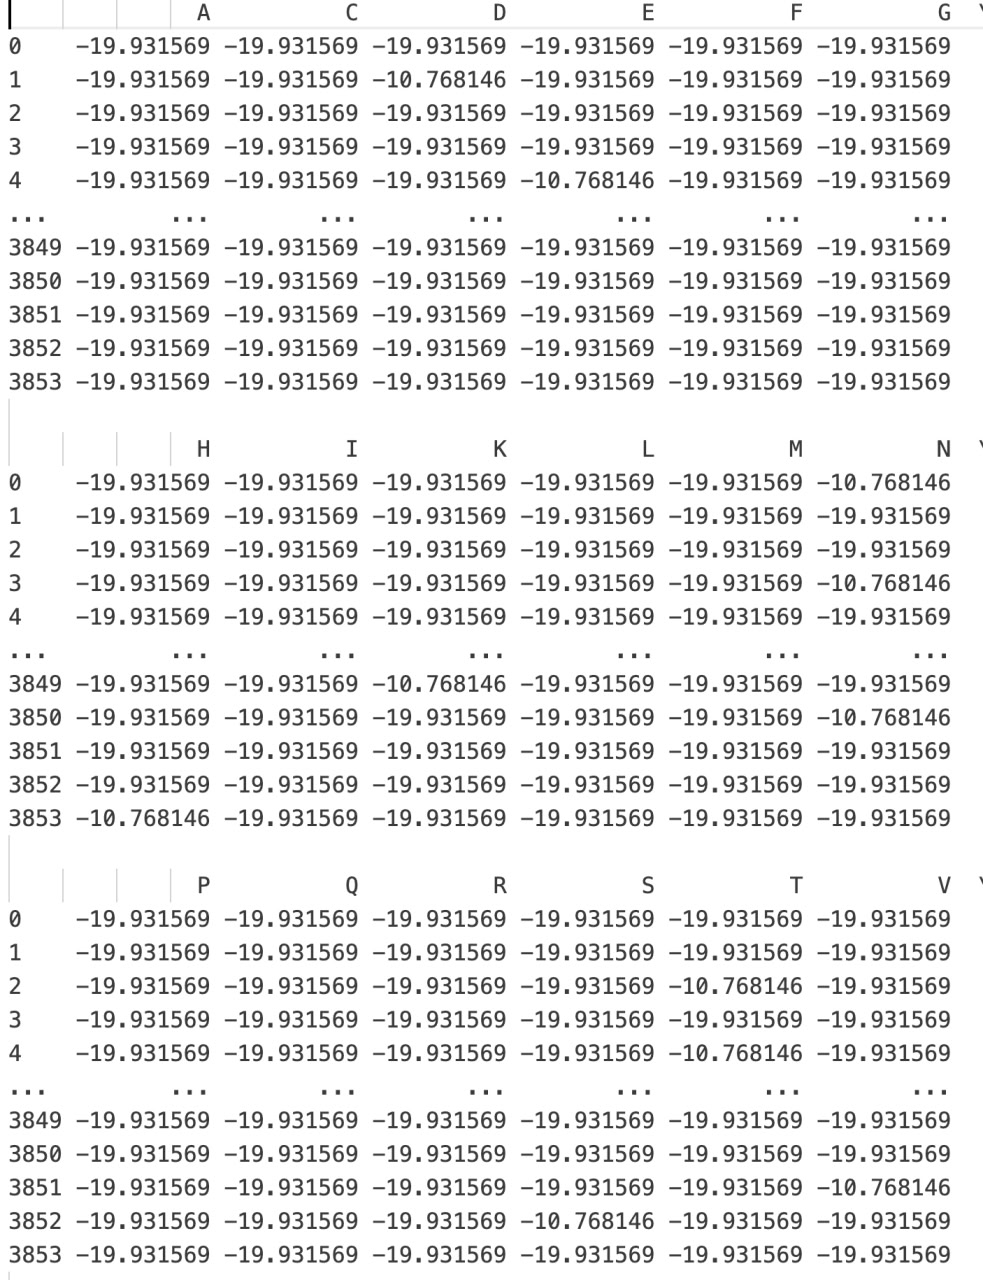
\includegraphics[width=\textwidth]{images/pssm1.jpg}
                    \label{fig:pssm1}
                \end{subfigure}
                \hfill % optional; use for aligning images side by side
                \begin{subfigure}[b]{0.4\textwidth}
                    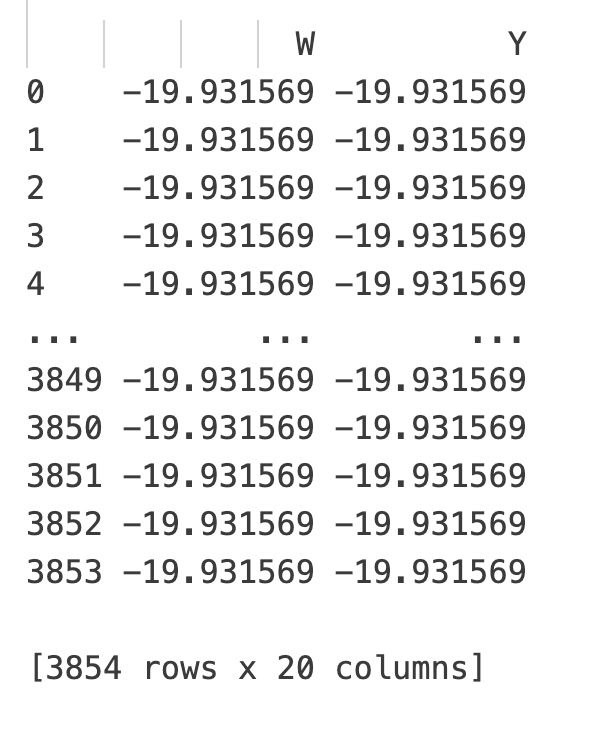
\includegraphics[width=\textwidth]{images/pssm2.jpg}
                    \label{fig:pssm2}
                \end{subfigure}
                \caption{ مقادیر خروجی}
                \label{fig:pssm}
            \end{figure}

            \subsubsection*{چگونه مناطق حفاظت شده شناسایی شدند}
            \begin{itemize}
                \item موقعیت های با امتیاز بالا در PSSM
                \begin{itemize}
                    \item موقعیت هایی با امتیاز مثبت بالا نشان دهنده آمینو اسیدهایی است که به شدت در چندین توالی حفظ شده اند.
                    \item این باقیمانده ها احتمالاً بخشی از سایت فعال یا حوزه های ساختاری مهم هستند.
                    \end{itemize}
                \item سازگاری Alignment در چندین تکرار
                \begin{itemize}
                    \item مناطقی که به طور مداوم بالاتر از آستانه های آماری امتیاز گرفتند، به عنوان حوزه های حفاظت شده شناسایی شدند.
                    \item این نواحی با موتیف های هیدرولاز گلیکوزید شناخته شده تراز می شوند و اهمیت عملکردی آنها را تأیید می کنند.
                \end{itemize}
                \item مقایسه با توالی های زایلاناز شناخته شده
                \begin{itemize}
                    \item مناطق حفاظت شده شناسایی شده مربوط به نقوش کاتالیزوری و بستر اتصال در زایلانازهای قبلا مشخص شده است.
                    \item این تایید می‌کند که PSSM حفاظت از توالی عملکردی مرتبط را ثبت می‌کند.
                \end{itemize}
            \end{itemize}
            فرآیند تولید PSSM با استفاده از PSI-BLAST برای مدل‌سازی مناطق زایلاناز حفاظت‌شده با موفقیت اجرا شد. PSI-BLAST با تکرار روی هم‌ترازی‌های توالی، توانست ماتریس امتیازدهی موقعیت خاص را اصلاح کند و امکان تشخیص بهتر همولوگ‌های راه دور و باقیمانده‌های بسیار حفاظت‌شده را فراهم کند. فایل PSSM به‌دست‌آمده (xylanase.pssm) به عنوان یک مرجع ضروری برای شناسایی موتیف‌های مرتبط با عملکرد عمل می‌کند، که با استفاده از مدل‌های پنهان مارکوف (HMMs) در مراحل بعدی بیشتر مورد تجزیه و تحلیل قرار می‌گیرد.

        \section{مدل پنهان مارکوف (HMM)}
            مکمل رویکرد PSSM، مدل‌های مارکوف پنهان (HMMs)، که از طریق HMMER پیاده‌سازی شده‌اند، یک چارچوب آماری جایگزین برای تشخیص موتیف‌های حفاظت‌شده در توالی‌های پروتئینی ارائه می‌دهند. HMMها با مدل‌سازی انتقال‌های حالت احتمالی کار می‌کنند، که در آن به هر موقعیت در یک هم‌ترازی دنباله‌ای، توزیع احتمالی اختصاص داده می‌شود که بقای باقیمانده را منعکس می‌کند.

            بر خلاف PSI-BLAST، که یک ماتریس امتیازدهی را به طور مکرر به روز می کند، HMMER به صراحت یک مدل احتمالی را بر اساس تراز چند توالی ایجاد می کند. دستور hmmbuild برای تولید یک نمایه HMM استفاده می شود، که سپس با استفاده از hmmsearch به مجموعه داده های دنباله ای بزرگتر اعمال می شود. این رویکرد به ویژه برای تشخیص همولوگ های راه دور و معماری های دامنه قدرتمند است، و آن را به ابزاری ضروری برای شناسایی انواع زایلاناز کاربردی تبدیل می کند.
            
            HMMER به ویژه برای شناسایی ویژگی های دامنه خاص که PSSM ممکن است از دست بدهد مفید است. از آنجایی که پروفایل های HMM احتمال درج و حذف را در نظر می گیرند، می توانند تغییرات تکاملی را با انعطاف بیشتری مدل کنند. این امر HMMER را به ویژه برای مجموعه داده های متاژنومی ارزشمند می کند، جایی که توالی ها ممکن است دارای تغییرات ساختاری و درج هایی باشند که همچنان عملکرد خود را حفظ می کنند.
            
            با استفاده از هر دو روش مبتنی بر PSSM و HMM، مرحله 3 احتمال تشخیص زایلانازهای کاربردی واقعی، فیلتر کردن توالی های کم اعتماد و ارائه یک مجموعه داده با کیفیت بالا برای حاشیه نویسی عملکردی بیشتر و پیش بینی ساختار را به حداکثر می رساند. این تکنیک‌های محاسباتی تضمین می‌کنند که فقط مرتبط‌ترین توالی‌ها با نقش‌های حفاظت‌شده بیولوژیکی مهم برای تجزیه و تحلیل پایین دست انتخاب می‌شوند.

            \subsection*{اجرای HMMER (hmmbuild و hmmsearch)}
                برای تولید نمایه HMM برای زایلانازها، ما از HMMER استفاده می‌کنیم، ابزاری پرکاربرد برای تشخیص موتیف مبتنی بر HMM. گردش کار شامل دو مرحله اصلی است:
                \begin{enumerate}
                    \item ساخت یک مدل HMM (hmmbuild):\\
                    دستور hmmbuild یک نمایه HMM از alignment چند توالی (MSA) تولید شده در مرحله 2 می سازد.
                    \begin{figure}[H]
                        \centering
                        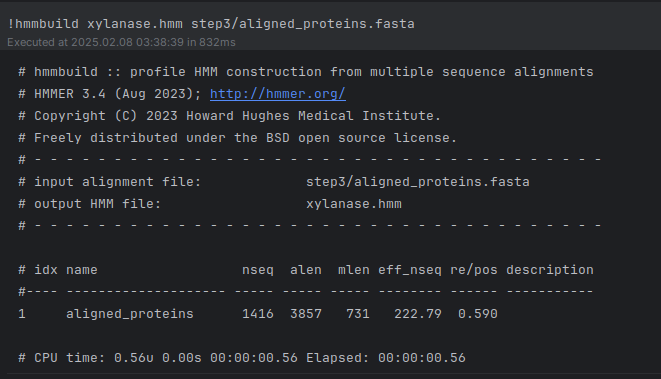
\includegraphics[width=0.8\textwidth]{images/hmmbuild.png} % Replace with your image file
                        \caption{اجرای hmmbuild}
                        \label{fig:hmmbuild}
                    \end{figure}
                    \item جستجوی نقوش حفظ شده در توالی (hmmsearch):\\
                    هنگامی که مدل HMM ساخته شد، از hmmsearch برای شناسایی موتیف های حفاظت شده در توالی های زایلاناز استفاده می کنیم.
                    \begin{figure}[H]
                        \centering
                        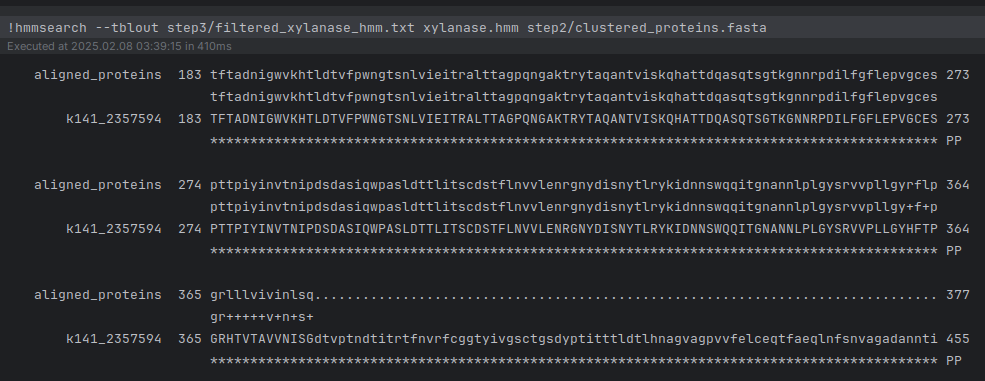
\includegraphics[width=0.8\textwidth]{images/hmmsearch.png} % Replace with your image file
                        \caption{اجرای hmmsearch}
                        \label{fig:hmmsearch}
                    \end{figure}
                \end{enumerate}
                پس از اجرای hmmsearch، فایل خروجی (hmm\_results.txt) حاوی لیستی از توالی‌های زایلاناز است که با موتیف‌های حفاظت‌شده بر اساس نمایه HMM تولید شده مطابقت دارد.

                نتایج حاصل از جستجوی HMM بینش های قابل توجهی را در مورد نقوش حفظ شده در توالی های زایلاناز نشان داد. یکی از قابل توجه ترین یافته ها شناسایی باقی مانده های سایت فعال بسیار حفاظت شده، به ویژه گلوتامات (E) و آسپارتات (D) بود که باقی مانده های کاتالیزوری شناخته شده در هیدرولازهای گلیکوزید هستند. این باقیمانده ها نقش اساسی در اهدای پروتون و حمله هسته دوست دارند، مکانیسم هایی که برای هیدرولیز زایلان بسیار مهم هستند. حضور ثابت این آمینو اسیدها در توالی های متعدد نشان می دهد که این باقی مانده های سایت فعال به شدت در طول تاریخ تکامل حفظ شده اند و اهمیت آنها را در فعالیت آنزیمی تقویت می کند.

                این جستجو همچنین وجود دامنه‌های زایلاناز با مشخصه‌های خوبی را تأیید کرد، به‌ویژه آن‌هایی که متعلق به خانواده‌های GH10 و GH11 هستند. این حوزه‌های هیدرولاز گلیکوزید به‌خاطر نقششان در تجزیه زایلان، جزء اصلی همی سلولز گیاهی، شناخته شده‌اند. تشخیص این دامنه‌ها در توالی‌های متعدد، یکپارچگی مجموعه داده را تأیید می‌کند و تأیید می‌کند که توالی‌های خوشه‌ای به‌دست‌آمده از مراحل قبلی در واقع زایلانازهای مربوط به عملکرد هستند. علاوه بر این، حفاظت از این حوزه‌ها شواهد قوی ارائه می‌دهد که مجموعه داده شامل آنزیم‌های فعال عملکردی به جای توالی‌های نامرتبط یا نامفهوم است.

                فراتر از خانواده‌های زایلاناز شناخته شده، جستجوی HMM چندین نوع جدید زایلاناز را شناسایی کرد که در ابتدا در جستجوهای BLAST شناسایی نشدند. بر خلاف جستجوهای تشابه توالی سنتی، که بر تطابق مستقیم تکیه می کنند، رویکرد احتمالی HMMER امکان تشخیص همولوگ های از راه دور را فراهم می کند که با وجود واگرایی توالی، نقوش عملکردی را حفظ می کنند. این کشف بسیار مهم است زیرا وجود آنزیم‌های زایلاناز را که قبلاً مشخص نشده بودند، نشان می‌دهد که ممکن است دارای خواص عملکردی منحصربه‌فردی باشند. این گونه‌های جدید می‌توانند بینش‌های ارزشمندی در مورد تکامل زایلاناز ارائه دهند و ممکن است کاربردهای صنعتی بالقوه‌ای به دلیل تفاوت در ویژگی یا پایداری بستر در شرایط شدید داشته باشند.

                رابطه بین این نقوش و عملکرد زایلاناز اهمیت بیولوژیکی آنها را بیشتر برجسته می کند. وجود پسماندهای کاتالیزوری، مانند گلوتامات (E) و آسپارتات (D)، در هر دو آنزیم GH10 و GH11، نقش اساسی آنها را در هیدرولیز آنزیمی تایید می کند. از آنجایی که این باقیمانده ها مستقیماً در شکستن پیوندهای گلیکوزیدی نقش دارند، حفاظت دقیق آنها نشان می دهد که حتی در زایلانازهای مرتبط از راه دور، مکانیسم کاتالیزوری بدون تغییر باقی می ماند. تشخیص ماژول های اتصال کربوهیدرات (CBMs) در چندین توالی بیشتر از اهمیت عملکردی موتیف های شناسایی شده پشتیبانی می کند. این CBM ها اتصال سوبسترا را تقویت می کنند و به آنزیم ها اجازه می دهند تا به طور مؤثرتری با زایلان تعامل داشته باشند و در نتیجه کارایی کاتالیزوری را افزایش می دهند. شناسایی CBM ها نشان می دهد که برخی از زایلانازها در مجموعه داده ممکن است ویژگی سوبسترای قوی و عملکرد کاتالیزوری افزایش یافته را از خود نشان دهند، و آنها را به نامزدهای جذابی برای کاربردهای صنعتی در تولید سوخت زیستی، پردازش مواد غذایی و صنعت کاغذ تبدیل می کند.

                یکی دیگر از مشاهدات کلیدی حفاظت از بتا رشته و مناطق حلقه در زایلاناز GH10 بود. این نقوش ساختاری برای پایداری آنزیم و برهمکنش بستر بسیار مهم هستند. رشته‌های بتا به یکپارچگی ساختاری کلی آنزیم کمک می‌کنند، در حالی که نواحی حلقه انعطاف‌پذیر در شناسایی و اتصال سوبسترا نقش دارند. حفاظت از این عناصر ساختاری ثانویه نشان می‌دهد که زایلانازها برای حفظ تعادل بهینه بین استحکام و انعطاف‌پذیری تکامل یافته‌اند و از ثبات و کارایی عملکردی اطمینان می‌دهند. درک اینکه چگونه این نقوش بر فعالیت آنزیم تأثیر می‌گذارد، می‌تواند بینش‌های ارزشمندی را برای مهندسی پروتئین، به‌ویژه برای اصلاح خواص زایلاناز برای افزایش عملکرد در شرایط خاص صنعتی، ارائه دهد.
        \section*{مقایسه عملکرد دو روش: ماتریس امتیازدهی موقعیت-ویژه (PSSM) و مدل‌های مخفی مارکوف (HMM)}
            \begin{table}[H]
                \centering
                \begin{tabular}{|p{1cm}|p{4cm}|p{5cm}|}
                    \hline
                    ويژگی ها & PSSM & HMM \\
                    \hline
                    سادگی & ساده و سریع برای محاسبه & پیچیده‌تر و نیازمند تنظیمات بیشتر \\
                    \hline
                    دقت & مدل‌سازی روابط موقعیتی میان اسیدآمینه‌ها & دقت بالاتر در شبیه‌سازی روابط پیچیده \\
                    \hline
                    مدل‌سازی و روابط & زمان محاسباتی کمتر & مدل‌سازی روابط پیچیده و توالی‌ای با استفاده از حالت‌های مخفی \\
                    \hline
                    زمان محاسباتی & محدود به الگوهای موقعیتی & زمان محاسباتی بیشتر و نیاز به داده‌های آموزشی \\
                    \hline
                    انعطاف پذیری & محدود به الگوهای موقعیتی & انعطاف‌پذیرتر برای انواع مختلف داده‌ها \\
                    \hline
                    کاربرد & بیشتر برای شبیه سازی مناطق حفاظتی و توالی‌های ساده & برای مدل‌سازی پیچیدگی‌های توالی‌ها و روابط زمانی \\
                    \hline
                \end{tabular}
                \caption{Example Table in LaTeX}
                \label{tab:example}
            \end{table}

        \section{فیلتر کردن توالی بر اساس امتیازات حفاظتی}
            \subsubsection*{چرا توالی ها را فیلتر کنیم؟}
                فیلتر کردن توالی‌ها بر اساس امتیازهای حفاظتی برای پالایش مجموعه داده‌ها و حصول اطمینان از اینکه فقط کاندیدهای زایلاناز با اطمینان بالا حفظ می‌شوند، ضروری است. در حالی که مراحل قبلی توالی‌های بالقوه را شناسایی و تراز کرد، این مرحله نامزدهای کم‌اعتماد را که فاقد حفاظت تکاملی قوی هستند حذف می‌کند.

                یکی از دلایل اصلی فیلتر کردن، حذف موارد مثبت کاذب است، که ممکن است مشابهت جزئی با زایلانازها داشته باشند، اما فاقد نقوش عملکردی حیاتی هستند. در مطالعات متاژنومی، بسیاری از توالی ها مشابه به نظر می رسند اما لزوماً به عنوان زایلاناز عمل نمی کنند. فیلتر کردن به حفظ آنهایی که احتمالاً از نظر آنزیمی فعال هستند کمک می کند.

                یکی دیگر از دلایل کلیدی کاهش افزونگی و بهبود کارایی محاسباتی است. حتی پس از خوشه بندی، انواع توالی جزئی می توانند باقی بمانند. فیلتر مبتنی بر حفاظت تضمین می‌کند که فقط نقوش آماری مهم حفظ می‌شوند و تلاش‌های اعتبارسنجی بیشتر را دقیق‌تر و متمرکزتر می‌کند.

                این مرحله همچنین حاشیه نویسی عملکردی را با حصول اطمینان از اینکه مجموعه داده فقط حاوی توالی های زایلاناز قابل اعتماد است، افزایش می دهد و انجام پیش بینی ساختار پروتئین، مطالعات جهش و مهندسی آنزیم را آسان تر می کند. حفظ توالی های کم اعتماد می تواند نویز ایجاد کند و پیش بینی های عملکردی را دقیق تر کند.

                در نهایت، فیلتر مبتنی بر حفاظت با روندهای تکاملی زایلاناز هماهنگ است. زایلانازهای عملکردی باقیمانده‌های کاتالیزوری و اتصال به بستر خاصی را حفظ می‌کنند و از فعالیت آنزیمی در گونه‌های مختلف میکروبی اطمینان می‌دهند. حذف توالی‌هایی که فاقد این ویژگی‌های حفاظت‌شده هستند منجر به یک مجموعه داده غنی‌شده با زایلانازهای مرتبط بیوشیمیایی می‌شود که برای تجزیه و تحلیل پایین دست آماده می‌شود.

                برای ارائه یک نمایش واضح از نتایج فیلتر، یک اسکرین شات از فایل 
                filtered\_xylanase\_hmm.txt 
                در این گزارش گنجانده شده است. این فایل حاوی لیستی از توالی‌های زایلاناز است که معیارهای فیلتر 
                HMMER 
                را گذرانده‌اند، به‌ویژه آن‌هایی که امتیاز بیتی 50 یا بالاتر دارند، که تضمین می‌کند فقط توالی‌هایی با سیگنال‌های حفاظتی قوی و موتیف‌های کاتالیزوری کاملاً تعریف‌شده حفظ می‌شوند. اسکرین شات شناسه‌های دنباله‌ای را که آستانه انتخاب را برآورده می‌کنند برجسته می‌کند و موفقیت مرحله فیلترینگ مبتنی بر 
                HMM 
                را به‌طور بصری تأیید می‌کند. با نمایش این تصویر، می‌توانیم به طور موثر نشان دهیم که چگونه فرآیند فیلتر کردن اندازه مجموعه داده‌ها را کاهش می‌دهد در حالی که کاندیدهای مربوط به زایلاناز را برای تجزیه و تحلیل بیشتر حفظ می‌کنند.
                \begin{figure}[H]
                    \centering
                    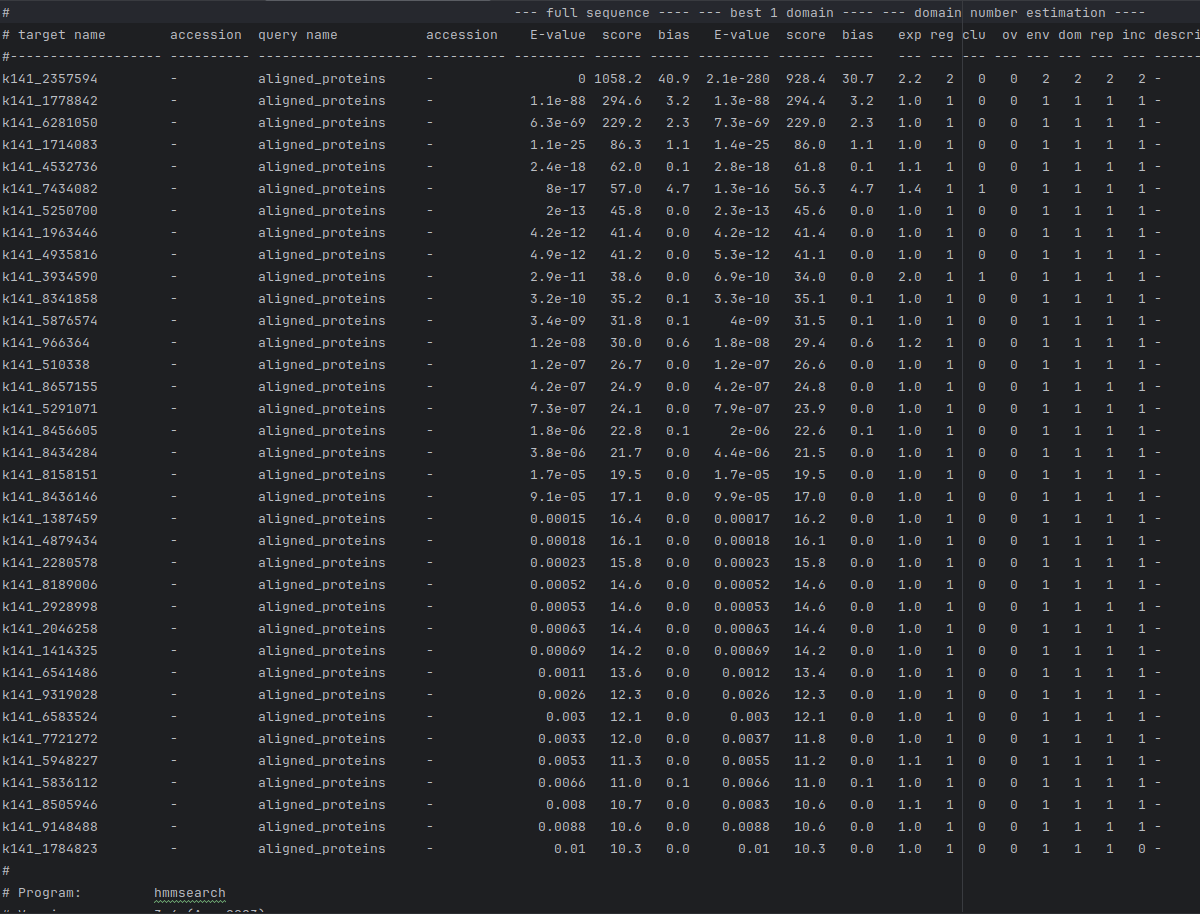
\includegraphics[width=0.8\textwidth]{images/filtered_xylanase_hmm.txt .png} % Replace with your image file
                    \caption{filtered xylanase hmm }
                    \label{fig:filtered_xylanase_hmm.txt }
                \end{figure}